\documentclass[class=book, crop=false]{standalone}
\usepackage[subpreambles=true]{standalone}
\usepackage{/home/mark/Documents/gradschool/research/thesis/preamble}
\usepackage{import}

\begin{document}

\chapter{Exceptional Cases}
In the previous chapter we were able to show that $\U$ is not finitely generated for a large family of Weyl groups $W$ with labels $a\le b\le c.$ These results were based on assuming $b\ge 4$ which allowed us to show that $\D$ was infinite and proceed from there. In fact, we didn't even describe all of the chambers in $\D,$ just an infinite family. However, the same approach will not work in the remaining cases because of the following lemma.
\begin{lemma} If $W$ is the Weyl group of $\G$ with labels $a\le b\le c$ as before, then $\D=\alpha_1\cap \alpha_n\cap \beta\cap \beta'$ as defined in the previous chapter is infinite if and only if $b\ge 4.$
	\label{infD}
\end{lemma}
\begin{proof}
	We know by Lemma \ref{infmany} that $\D$ is infinite if $b\ge 4.$ Thus it remains to show that $\D$ is finite if $b=3.$ If $b=3$ then $a=3$ also, and by definition of $a,b,c$ this means $m(s,t)=m(s,u)=3.$ We will also recall the definition of $\D=\alpha_1\cap \alpha_n\cap \beta \cap \beta'$ where
	\begin{align*}
	\alpha_1&=\{D\in \Sigma|d(D,C)<d(D,tC)\}=\{w\in W|\ell(w)<\ell(tw)\}\\
	\alpha_n&=\{D\in \Sigma|d(D,C)<d(D,uC)\}=\{w\in W|\ell(w)<\ell(uw)\}\\
	\beta&=\{D\in \Sigma|d(D,tC)<d(D,tsC)\}=\{w\in W|\ell(tw)<\ell(stw)\}\\
	\beta'&=\{D\in \Sigma|d(D,uC)<d(D,usC)\}=\{w\in W|\ell(uw)<\ell(suw)\}
\end{align*}

Let $w\in W$ and suppose $\ell(w)\ge 2.$ Then we can write $w=s_1s_2w'$ where $\ell(w')=\ell(w)-2.$ If $s_1=t$ then we have
\[
	\ell(tw)=\ell(s_2w')=\ell(w)-1<\ell(w)
\]
which shows $w\not\in \alpha_1$ and thus $w\not\in \D.$ A similar argument shows that $w\not\in \D$ if $s_1=u.$

Now we assume $s_1=s$ and so we can also assume $s_2=t,u.$ First let $s_2=t$ so that $w=stw'.$ If $w\not\in \alpha_1$ then $w\not\in \D$ and so wewill suppose $w\in\alpha_1.$ Now we can see
\[
	\ell(stw)=\ell(ststw')=\ell(sstsw')=\ell(tsw')\le \ell(w')+2=\ell(w)<\ell(tw)
\]
and thus $w\not\in \D.$ A similar argument shows that $w\not\in \D$ if $s_2=u.$

We have shown that if $\ell(w)\ge 2$ then $w\not\in \D$ and thus $\D$ must be finite as desired. In fact, if $a=b=3$ then we can check relatively easily that $\D=\{C,sC\}$ which proves the desired result.
\end{proof}

The previous lemma shows that generating results for the remaining cases is not just a matter of being slightly more clever when we look for vertices, but changing the strategy as a whole. In fact, in some cases our proof strategy needs to switch entirely since $\U$ will be finitely generated in some cases as we will see. First, we will show which of the remaining cases are not finitely generated.

\section{Case: 336 over $\F{2}$}
We saw in the previous chapter that a vertex contained in $\D$ was a sufficient condition to construct a corresponding map $\tilde{\phi_v}.$ However, it is not a necessary condition, and we will see in this section we can relax a few conditions to still construct $\tilde{\phi_v}$ for infinitely many vertices. Our first step is to make some general observations about this case and then prove a statment similar to Lemma \ref{existence}.

For the remainder of the section, $\G$ will be the Kac-Moody group over $\F{2}$ with Weyl group defined by a the 336 Coxeter diagram, and $\U$ will be its unipotent subgroup. To be more precise we will say $W=\langle s,t,u|s^2=t^2=u^2=(st)^3=(su)^3=(tu)^6=1\rangle.$ The rest of our assumptions will be the same as in the previous chapter.

For any positive root $\alpha$ of $\Sigma,$ we know that $\U_\alpha\cong (\F{2},+)$ and thus each $\U_\alpha$ is a cyclic group of order 2. This means we can let $u_\alpha$ be the non-identity element of $\U_\alpha$ for all $\alpha\in \Phi^+.$ Then we know that $\U$ is generated by $\{u_\alpha\}$ for all $\alpha\in \Phi^+$ and there are exactly 3 types of relations:
\begin{align*}
	u_\alpha^2&=1&&\text{For all }\alpha\in \Phi^+\\
[u_\alpha,u_\beta]&=1&&\text{if }\partial\alpha\cap \partial\beta=\emptyset\\
[u_\alpha,u_\beta]&=w&&\text{where }w\text{ is a word in }\U_{(\alpha,\beta)}\subset \U_y\text{ where }y=\partial\alpha\cap \partial\beta
\end{align*}
Note that is presentation is the same as that in the previous chapter, just slightly simplified since we know precicely which field $k$ we are working with now.

Let $v$ be any vertex of $\Sigma$ of type $s,$ meaning $|\st(v)|=12.$ Then we showed previouly that there is a map $\phi_v:\U_v\to K$ where $K$ is a cyclic group of order 2. If we label the positive roots through $v$ as  $\gamma_1,\dots,\gamma_6$ with $\gamma_i\cap \gamma_j\subset \gamma_k$ for $1\le i\le k\le j\le 6,$ then we also know that at least one of $\U_{\gamma_2}$ or $\U_{\gamma_5}$ must be sent to the identity by $\phi_v.$ By reversal of the numbering, we can assume without loss of generality that $\phi(\U_{\gamma_5})=1.$ As in the previous chapter we want to define an extension of $\phi_v$ to a map $\tilde{\phi_v}:\U\to K.$ We define this extension by
\[
	\tilde{\phi_v}(u_\alpha)=\begin{cases}\phi_v(u_\alpha)&\text{if }v\text{ lies on }\partial\alpha\\1&\text{otherwise}
	\end{cases}
	\]
	Since we have defined $\tilde{\phi_v}$ for all generators, to check it is well defined is a matter of checking the relations in our presentation.To this end we have to following lemma. Again note that this is the same definition as in Lemma \ref{existence}, simply stated in terms of our new, simplified presentation.

	\begin{lemma} Let $v$ be a vertex of $\Sigma$ of type $s,$ meaning $|\st(v)|=12,$ and let $\gamma_1,\dots,\gamma_6$ be the positive roots through $v,$ labeled as before. Also suppose that $\phi_v(\U_{\gamma_5})=1.$ If $\gamma_2,\gamma_3,$ and $\gamma_4$ are simple at all other vertices they meet, then $\tilde{\phi_v}$ as defined in Lemma \ref{existence} exists.
	\label{336f2existence}
\end{lemma}
\begin{proof}
	To check $\tilde{\phi_v}$ is well defined is a matter of checking the relations are satisfied by the images under $\tilde{\phi_v}.$ Since $\tilde{\phi_v}$ has a cyclic group of order 2 as its codomain, we can see immediately that the first two types of relations will be satisfied regardless of $\alpha$ and $\beta.$ Now to check the third type.

	Suppose $\alpha$ and $\beta$ are any two positive roots with $y=\partial\alpha\cap \partial\beta.$ Since $[u_\alpha,u_\beta]$ must be mapped to the identity then we just need to check that $w$ is also mapped to the identity. If $y=v$ then $u_\alpha,u_\beta,w$ all lie in $\U_v$ and $\tilde{\phi_v}(w)=\phi_v(w)$ which must be the identity because $\phi_v$ is a well defined homomorphism.

	Now suppose $y\neq v.$ Let $\delta_1,\dots,\delta_n$ be the positive roots through $y,$ labeled as normal, and assume that $\alpha=\delta_i$ and $\beta=\delta_j$ with $i<j.$ There is at most one positive root whose wall can pass through both $v$ and $y,$ call it $\delta_k$ if it exists. If $\delta_k$ does not exist, then no positive roots through $y$ pass through $v$ and so $\tilde{\phi_v}(u_{\delta_m})=1$ for all $m.$ Thus $\tilde{\phi_v}(w)=1$ as desired.

	Now suppose $\delta_k$ does exist and $\delta_k=\gamma_r$ for $r\in \{1,5,6\}.$ Then we know $\tilde{\phi_v}(u_{\delta_m})=1$ for all  $m\neq k$ and $\tilde{\phi_v}(u_{\delta_k})=\tilde{\phi_v}(u_{\gamma_r})=\phi_v(u_{\gamma_r})=1$ by the construction of $\phi_v.$ Thus $\tilde{\phi_v}(u_{\delta_m})=1$ for all $m$ and so $\tilde{\phi_v}(w)=1$ as well.

	Now suppose $\delta_k$ does exist and $\delta_k=\gamma_r$ for $r\in \{2,3,4\}.$ Then by assumption, $\delta_k$ is simple at $y$ and thus $k=1,n.$ Thus $\tilde{\phi_v}(u_{\delta_m})=1$ for all $2\le m\le n-1.$ But $w$ is a word in $\U_{(\alpha,\beta)}\subset \U_{(\delta_2,\delta_{n-1})}$ and thus $\tilde{\phi_v}(w)=1$ again, which gives the result.
\end{proof}

It is worth noting that the hypotheses of this Lemma are weaker than those of Lemma \ref{existence}, and so we have a hope of constructing more $\tilde{\phi_v}$ then the theory of the previous chapter would allow us to. However, many of the ideas will still be similar and the proofs in this section will run parallel to those in the previous chapter.

Let $x$ be the vertex of $C$ of type $s$ as in the previous chapter and let $\alpha_1,\dots,\alpha_6$ be the positive roots through $x,$ labeled as usual. Also assume without loss of generality that $\phi_x(u_{\alpha_5})=1.$ Now let $\D'=\alpha_1\cap \alpha_6\cap \beta$ where $\beta$ is defined as in the previous chapter. We can now prove a lemma similar to Lemma \ref{containD}.\\
\Huge picture of $\D'$\normalsize\\

\begin{lemma}
	\label{336f2containD}
	Let $x$ be the vertex of $C$ of type $s$ so that $|\st(x)|=12.$ Let $\alpha_1,\dots,\alpha_6$ be the positive roots at $x$ with the standard ordering. Also assume that $\phi_x(\U_{\gamma_5})=1.$ Suppose $\gamma=\alpha_i$ for $i\in \{2,3,4\}.$ If $\delta$ is any positive root with $\partial\gamma\cap \partial\delta\neq \emptyset$ then $\D'=\alpha_1\cap \alpha_6\cap \beta\subset \gamma\cap \delta$ where 
	\[
	\beta=\{D\in \Sigma|d(D,tC)<d(D,tsC)\}=\{w\in W|\ell(tw)<\ell(stw)\}
	\]
	as in the previous chapter.
\end{lemma}
\begin{proof}
	By assumption, $\gamma$ is a positive root through $x$ and thus we have $\D'\subset \alpha_1\cap \alpha_6\subset \gamma.$ Thus it remains to show that $\D'\subset \delta.$

	Let $y=\partial\gamma\cap \partial\delta.$ If $y=x$ then $\delta$ is also a positive root through $x$ and so $\D'\subset \delta$ as desired. Now suppose $y\neq x.$ Then there are two cases to consdier. First suppose that $\partial \delta$ does not meet $\partial\alpha_1$ or $\partial\alpha_6.$ Then arguments identical to those made in Lemma \ref{containD} show that $\D'\subset \alpha_1\cap \alpha_6\subset \delta$ as desired.

Now suppose that $\partial\delta$ does meet $\alpha_1$ or $\alpha_6$ at a point $y'$ which cannot be $x$ as $\delta\neq \gamma.$ Then the vertices $x,y,y'$ form a triangle which must be a chamber, call it $C',$ by the triangle condition. This chamber will have a vertex of $x$ and a vertex on $\partial\alpha_1$ or $\partial\alpha_6$ and thus $C'$ is either $C,tC,$ or $uC.$ But none of the vertices of $C$ or $uC$ lie on $\partial\alpha_i$ for $2\le i\le 4$ and thus $C'$ must be $tC.$ But then $\gamma=\alpha_2$ and $\delta=\beta$ by definition and thus $\D'\subset \beta'=\delta$ as desired.
\end{proof}

The proofs in the previous chapter relied heavily on facts about simple roots, and to aid these proofs we had Lemma \ref{preservesimple} which shows the $W$ action on $\Sigma$ preserves simplicity under certain condidtions. Now that we are dealing more than just simple roots we need to extend this lemma to the current context.

\begin{lemma}
	\label{preservemapto1}
	Suppose $v$ is a vertex of $\Sigma$ of type $s$ so that $\U'_v\neq \U_v,$ and $w\in W$ such that $w\gamma$ is a positive root at $wv$ for all positive roots $\gamma$ at $v.$ If $\delta$ is a positive root at $v$ such that $\phi_v(u_\delta)=1$ then $\phi_{wv}(u_{w\delta})=1$ as well.
\end{lemma}
\begin{proof}
	We know from the theory of Moufang twin buildings that there is some $\tilde{w}\in \mathrm{Aut}(\Delta)$ such that $\tilde{w}\U_\alpha\tilde{w}^{-1}=\U_{w\alpha}$ for all roots $\alpha\in \Phi.$ Let $\psi_w:\G\to \G$ be the conjugation isomorphism defined by $\tilde{w}.$ For any positive root $\gamma$ at $v,$ we know $w\gamma$ is positive at $wv$ by assumption, and thus $\psi_w(u_\gamma)=u_{w\gamma}\in \U_{w\gamma}.$ Thus the map $\psi_w$ restricts to a map from $\U_v$ to $\U_{wv}$ which is necessarily injective. Now suppose $\gamma'$ is a positive root at $wv.$ There are only finitely many roots at $v$ and $wv,$ and since $w$ sends positive roots to positive roots, it must also send negative roots to negative roots. Thus $w^{-1}$ must also send positive roots at $wv$ to positive roots at $v.$ Thus $w^{-1}\gamma'$ is a positive root at $v.$ Thus $\psi_w(u_{w^{-1}\gamma'})=\gamma'$ which means $\psi_w:\U_v\to \U_{wv}$ is surjective and thus an isomorphism.

	Now consider the map $f=\phi_{wv}\psi_w:\U_v\to K.$ We know $\psi_w$ is an isomorphism, and $\phi_{wv}$ is surjective and thus $f$ is surjective. By Lemma \ref{preservesimple} we know that if $\gamma$ is simple at $wv$ then $w^{-1}\gamma$ is simple at $v$ and $f(u_{w^{-1}\gamma})=\phi_{wv}(\gamma)=1$ by the definition of $\phi_{wv}.$ Thus if $\U_1,\U_6$ are the simple roots at $v$ then $\U_1,\U_6\le \ker f.$ Thus $\ker f$ is a normal subgroup of $\U_v$ containing $\U_1$ and $\U_6$ so $\ker f=\ker \phi_v$ by Lemma \ref{uniquephiv}.

	Since $\psi_w$ is an isomorphism we know $\ker \phi_{wv}=\psi_w(\ker f)=\psi_w(\ker \phi_{v})$ and thus if $u_\delta\in \ker \phi_v$ then $\psi_w(u_\delta)=u_{w\delta}\in \ker \phi_{wv}$ which gives the desired result.
\end{proof}

Another way of viewing this lemma is as follows. The local homomorphisms $\phi_v$ assign the two simple roots at $v$ to the short and long roots of a root system of type $G_2,$ depeding on which other roots are sent to the identity. We cannot tell just from the information of the Coxeter complex which way this assignment will be. However, we have just proved that the $W$ action respects this assignment. We have essentially proved that if $\alpha$ is a long root at $v,$ then under suitable conditions, $w\alpha$ is a long root at $wv.$ We are now prepared to prove a new result corresponding to Lemma \ref{Dexists}.

\begin{lemma} 
	Let $x$ be the vertex of $C$ of type $s$ and label the positive roots at $x$ as $\alpha_1,\dots,\alpha_6$ with the standard ordering in such a way that $\phi_x(\U_{\alpha_5})=1.$ If $v=w^{-1}x\in \D'=\alpha_1\cap \alpha_6\cap \beta$ with then $\tilde{\phi}_{wx}$ as defined in Lemma \ref{existence} exists. Recall from the previous chapter that 
	\[
	\beta=\{D\in \Sigma|d(D,tC)<d(D,tsC)\}=\{w\in W|\ell(tw)<\ell(stw)\}
\]
	\label{336f2Dexists}
\end{lemma}
\begin{proof}
	The proof will proceed in a manner very similar to the proof of Lemma \ref{Dexists}. Let $D=\mathrm{Proj}_{w^{-1}x}(C)$ and let $D=(w')^{-1}C.$ By the definition of projections, $w^{-1}x$ is a vertex of $D$ of type $s,$ but $(w')^{-1}x$ is also a vertex of $D$ of type $s,$ and thus $(w')^{-1}x=w^{-1}x.$ Now without loss of generality we may assume that $w'=w.$ Again, the definition of projections means that $D$ is the closest vertex to $C$ which has a vertex of $w^{-1}x.$ Since $\mathcal{D}$ is convex, and $w^{-1}x$ and $C$ both lie in $\mathcal{D},$ we also know that $D=\mathrm{Proj}_{w^{-1}x}(C)$ lies in $\mathcal{D}$ as well. By a similar argument we know that $\mathrm{Proj}_{x}(D)$ must lie in $\mathcal{D}\subset \alpha_1\cap \alpha_n$ and thus $\mathrm{Proj}_{x}(D)=C.$ Now define $E=wC$ and note that the action of $W$ respects projections and thus we have
	\[
		E=wC=\mathrm{Proj}_{wx}{wD}=\mathrm{Proj}_{wx}{C} \qquad C=wD=\mathrm{Proj}_{w(w^{-1}x)}{wC}=\mathrm{Proj}_{x}{E}
	\]
In particular, if $\gamma$ is any positive root through $wx$ then $E\in \gamma$ by the properties of projections.

Recall that the positive roots through $x$ are $\alpha_1,\dots,\alpha_6$ and we assumed that $\phi_x(u_{\alpha_5})=1.$ For any posititive root through $x,$ say $\alpha_i,$ we know that $D\in \alpha_i$ and thus $C=wD\in w\alpha_i.$ We also know $w\alpha_i$ will be a root through $wx$ and thus $w\alpha_i$ is a positive root through $x.$ Since $w$ sends positive roots at $x$ to positive roots at $wx$ we can use Lemma \ref{preservesimple} and Lemma \ref{preservemapto1}.

Now we can label the positive roots at $wx$ as $\gamma_1,\dots,\gamma_6$ in such a way that $\gamma_i=w\alpha_i$ for all $i.$ We need to check that this labeling satisfies all of the properties we normally use for labeling the positive roots through a vertex. If $1\le i\le k\le j\le 6$ then we know $\alpha_i\cap \alpha_j\subset \alpha_k$ and thus $w\alpha_i\cap w\alpha_j\subset w\alpha_k$ which shows $(\gamma_i,\gamma_j)=\{\gamma_k|i<k<j\}$ as desired. We also know by Lemma \ref{preservemapto1} that $\phi_{wx}(u_{\gamma_5})=1.$ 

Now we can try to apply Lemma \ref{336f2existence} to show $\tilde{\phi_{wx}}$ exists. Consider $\gamma_i$ for $2\le i\le 4.$ Let $y\neq wx$ be any other vertex on $\partial\gamma_i.$ If we apply $w^{-1}$ we get that $w^{-1}y\neq x$ is a vertex on $\alpha_i$ and thus $\alpha_i$ is simple at $w^{-1}y$ by Lemma \ref{positiveeverywhereelse}. Now suppose $\delta$ is any positive root at $w^{-1}y.$ Then $D\in \D'\subset \delta$ by Lemma \ref{336f2containD} and so $C,D\in \delta.$ But this means that $E,C\in w\delta$ and thus $w\delta$ is a positive root at $y.$ So $w$ sends positive roots at $w^{-1}y$ to positive roots at $y,$ and so by Lemma \ref{preservesimple} it must also send simple roots at $w^{-1}y$ to simple roots at $y.$ Since $\alpha_i$ is simple at $w^{-1}y$ then $\gamma_i$ is simple at $y$ as desired, and $\tilde{\phi_{wx}}$ exists by Lemma \ref{336f2existence}.

\end{proof}

As in the previous chapter, we now have a potentially large class of vertices for which $\tilde{\phi}_v$ exists, but we still must show there are infinitely many, and that they do not lie on finitely many walls. In fact, we can even use the same vertices as in the previous chapter. Let $w_k=(sut)^k$ for all $k\ge 0$ and let $v_k=w_kx.$ Recall in our current setup that $m(t,u)=6$ and $m(s,u)=m(s,t)=3.$ 

\begin{lemma}
	\label{336f2infmany}
	Let $w_k=(sut)^k$ for all $k\ge 0$ and let $x$ be the vertex of $C$ of type $s.$ Then the vertices $w_kx$ are all distinct, and they all lie in $\D'=\alpha_1\cap \alpha_6\cap\beta$ as defined previously.
\end{lemma}
\begin{proof}
	Many of the proofs will be identical to those in the proof of Lemma \ref{infmany} and so work will not be repeated when unnecessary. We can check that $\ell(w_k)=3k$ and $\ell(tw_k)=3k+1$ by identical arguments as before. We can also check that
	\begin{align*}
		uw_k&=u(sutsut\cdots)\\
		    &=(usu)(tsutsu\cdots)\\
		    &=(sus)(tsutsu\cdots)\\
		    &=(su)(sts)(utsuts\cdots)\\
		    &=(su)(tst)(utsuts\cdots)\\
		    &=(su)(ts)(tut)(sutsut\cdots)\\
	\end{align*}
We have exhausted all possible Coxeter relations in $uw_k$ and none of them led to a reduction in length so we can conclude that $\ell(uw_k)=3k+1$ also so that $w_k\in \alpha_1\cap \alpha_6.$

Now we do the same analysis for $stw_k$ to see
\begin{align*}
	stw_k&=st(sutsut\cdots)=(sts)(utsuts\cdots)\\
	     &=(tst)(utsuts\cdots)=(ts)(tut)(sutsut)\\
\end{align*}
and since no reductions can be performed we also get $\ell(stw_k)=3k+2$ so that $w_k\in \beta$ as well. Thus each $v_k$ lies in $\D'$ as desired. Each $v_k$ is unique by an identical argument as in Lemma \ref{infmany}.
\end{proof}

The last major step is to show that the $w_k^{-1}x$ cannot somehow lie on only finitely many walls. The analysis here will be slightly more complicated, but ultimately similar to that done in the previous chapter.

\begin{lemma}
	\label{336f2finitewalls}
	Let $x$ be the vertex of $C$ of type $s$ and let $w_k=(sut)^k$ for all $k\ge 0.$ Any wall of $\Sigma$ can contain only finitely many $w_k^{-1}x.$
\end{lemma}
\begin{proof}
	By arguments identical to those before, $w_m^{-1}x$ and $w_{n}^{-1}x$ will lie on the same wall if and only if $x$ and $v_k$ lie on the same wall for some $k\ge 0,$ and this will only happen if and only if either $w_k^{-1}uw_k$ or $w_k^{-1}tw_k$ lies in $\langle u,t\rangle.$ We will again apply the Coxter relations to show this is impossible for infinitely many $k.$ First we check
\begin{align*}
	w_k^{-1}tw_k&=(\cdots tustus)t(sutsut\cdots)\\
		    &=(\cdots tustu)(sts)(utsut\cdots)\\
		    &=(\cdots tustu)(tst)(utsut\cdots)\\
		    &=(\cdots tus)(tut)(s)(tut)(sut\cdots)
\end{align*}
and the we see also
\begin{align*}
	w_k^{-1}uw_k&=(\cdots stustus)u(sutsuts\cdots)\\
		    &=(\cdots stust)(ususu)(tsuts\cdots)\\
		    &=(\cdots stust)(s)(tsuts\cdots)\\
		    &=(\cdots stu)(ststs)(uts\cdots)\\
		    &=(\cdots stu)(t)(uts\cdots)\\
		    &=(\cdots stustu)(t)(utsuts\cdots)\\
		    &=(\cdots stus)(tutut)(suts\cdots)\\
\end{align*}
Now in the second case we were able to do some reductions so it is possible that $w_{k}^{-1}uw_k\in \langle s,t \rangle$ for small $k,$ but as long as $k$ is large enough, say $k\ge 3$ then this is no longer a possibility as we showed no further reductions are possible. Thus $w_m^{-1}x$ and $w_n^{-1}x$ can only lie on the same wall if $|n-m|\le 3.$

\end{proof}

Now we are ready to prove the main result of the section, which is nearly identical to the proof of Theorem \ref{notfinitelygenerated}.
\begin{theorem}
	\label{336f2notfg}
	Let $\G$ be the Kac-Moody group over $\F{2}$ with Weyl group defined by the edge labels $3,3,6.$ Then $\U$ is not finitely generated.
\end{theorem}
\begin{proof}
	Suppose that $\U$ is finitely generated. Then there is some finite set of roots $\beta_1,\dots,\beta_m$ such that $\U=\langle \U_{\beta_i}|1\le i\le m\rangle.$ Now only finitely many of the vertices $w_k^{-1}x$ lie on the same wall and thus we can choose $k$ so that $v=w_k^{-1}x$ does not lie on $\partial \beta_i$ for any $i.$ By Lemma \ref{336f2infmany} we know that $\tilde{\phi_v}$ exists, and by definition it is a surjective map from $\U\to C.$ However, we can also see by definition that $\tilde{\phi_v}(\U_{\beta_i})=1$ for all $i,$ since none of these walls meet $v.$ But this means $\tilde{\phi_v}$ sends all of the generators of $\U$ to the identity and thus it must be the trivial map which is a contradiction. Thus $\U$ is not finitely generated as desired.
\end{proof}

\section{Finite Generation in the Exceptional Cases}
Now there are two cases left to consider, and no ammount of modification to our previous strategies will work since we will see that these remaining cases are finitely generated. 

For any positive root $\gamma,$ we say that a chamber $D$ borders $\gamma$ if a panel of $D$ lies on $\partial \gamma.$ This allows us to define
\[
	d(\gamma,C)=\min_{D\text{ borders }\gamma} \{d(D,C)\}
\]
It is worth noting that if $d(\gamma,C)=k$ then there is a chamber $D$ which borders $\gamma$ and $d(\gamma,C)=d(D,C).$ Furthermore, the chamber $D$ must lie in $\gamma$ since, otherwise, the chamber adjacent to $D$ across $\partial\gamma$ would be closer to $C.$

We can now define $\U_n=\langle \U_{\gamma}|\gamma\in \Phi^+, d(\gamma,C)\le n$ which is a subgroup of $\U$ for all $n.$ We also have a few facts which are immediate from the definition of $\U_n.$ We can see that $\U_1\subset \U_2\subset \U_3\subset \cdots$ and $\U=\cup_{n}\U_n$ as any positive root will be some finite distance from $\C.$ 

Slightly less obvious is the fact that $\U_n$ is finitely generated for all $n.$ If $d(\gamma,C)\le n$ then ther must be a chamber $D$ which borders $\gamma$ with $d(D,C)\le n.$ There are only finitely many such chambers, and each of these chambers borders at most 3 roots, so $\U_n$ is finitely generated.

The idea of the remaining proofs will be to use the following lemma
\begin{lemma} 
	For any positive root $\gamma$ we define $d(\gamma,C)=\min\{d(D,C)|D\text{ has a panel on }\partial \gamma\}.$ Let $\U_n=\langle \U_\gamma |d(\gamma,C)\le n\rangle$ for all $n\ge 0$ where $d(\gamma,C).$ If there is some $N$ such that $\U_n\subset \U_{n-1}$ for $n>N$ then $\U$ is finitely generated.
	\label{fgcond}
\end{lemma}
\begin{proof}
	If $\U_n=\U_{n-1}$ for all $n> N$ then inductively we know that $\U_n=\U_N$ for all $n>N.$ Thus
	\[
		\U=\cup_{n=N}^{\infty}{\U_n}=\cup_{n=N}^\infty \U_N=\U_N
	\]
	which is fintely generated as desired.
\end{proof}

Since the remaining $W,k$ pairs the only exceptional cases in rank 3, it is clear that we will have to use not only the specific commutator relations of the local root groups, but also the geometry in the Coxeter complex specific to these choices of $W.$

\subsection{Case: 334 over $\F{2}$}
Before we start we will note that almost every case must be considered over $\F{2}$ and $\F{3},$ which ususally have to be done separately as there are difference in the commutator relations. However, a lack of a $6$ in the Coxeter diagram of $W$ means that $\U$ is finitely generated by the known theory for this choice of $W.$ Therefore, we will only consider this $W$ over $\F{2}.$

Let $W$ be the Coxeter group defined by a 334 diagram and $k=\F{2}.$ Then we will show $\U$ is finitely generated in this case.

\begin{theorem}
	\label{334f2fg}
	If $W=\langle s,t,u|s^2=t^2=u^2=(st)^3=(su)^3=(tu)^4=1\rangle$ and $k=\F{2}.$ Then $\U_n\subset \U_{n-1}$ for all $n>2.$
\end{theorem}
\begin{proof}
	Let $\gamma$ be any positive root with $d(\gamma,C)=n>2.$ Then choose a chamber $D_1$ which borders $\gamma$ such that $d(D_1,C)=d(\gamma,C).$ Now there is another chamber $D_2$ such that $D_1$ and $D_2$ are adjacent and $d(D_2,C)=d(D_1,C)-1.$ Then $D_1$ and $D_2$ will share exactly one vertex which lies on $\partial \gamma,$ call it $v.$ Recall that $\st(v)$ is the set of chambers of $\Sigma$ for which $v$ is a vertex. Then we have $|\st(v)|=6$ or $8.$

	First suppose $|\st(v)|=6.$ In $\Sigma,$ we can see that $\st(v)$ consists of the 6 chambers ``surrounding'' $v$ which each have a vertex on $v.$ Since we have already defined $D_1$ and $D_2$ we may label the other 4 chambers in $\st(v)$ as $D_3,\dots,D_6$ by going in a circular order around $v.$ Equivalently this means that $D_i$ is ajacent to $D_{i+1}$ for $1\le i\le 5$ and $D_6$ is also adjacent to $D_1.$ We also know that each positive root will contain exactly 3 of these vertices, and those three vertices will be $D_i,D_{i+1},$ and $D_{i+2}$ for some $i,$ where addition is done modulo 6.

	By construction, $D_2$ and $D_1$ are not adjacent along $\partial \gamma,$ but a panel of $D_1$ lies on $\partial \gamma,$ and thus $D_1$ and $D_6$ must be adjacent along $\partial\gamma.$ Since $D_6\not\in \gamma,$ this means that $\gamma$ must contain $D_1,D_2,D_3.$ Let $\alpha$ and $\beta$ be the other two positive roots through $v.$ We know that $\partial\gamma$ cannot separate $D_2$ and $D_1$ or $D_2$ and $D_3$ so we can say again without loss of generality that $\partial\alpha$ separates $D_2$ and $D_1$ while $\partial\beta$ separates $D_2$ and $D_3.$ 

	Now $D_3\in \gamma$ but $D_4\not\in \gamma$ which means that $D_3$ has a panel on $\partial\gamma.$ By our choice of $D_1$ we know that $d(D_3,C)\ge d(D_1,C)>d(D_2,C).$ We can conclude that $D_2\in \alpha\cap \beta\cap \gamma$ and thus $D_2=\proj_v(C).$ The local isomorphism at $v$ then gives $[\U_\alpha,\U_\beta]=\U_\gamma.$ However, we already showed that $D_2$ borders $\alpha$ and $\beta$ and $d(D_2,C)=d(D_1,C)-1=n-1$ so that $\U_\alpha,\U_\beta\in \U_{n-1}$ and thus $\U_\gamma\in \U_{n-1}$ as desired.\\
	\begin{figure}
		\label{deg6433f2}
		%\import{diagrams/}{deg6433f2}
		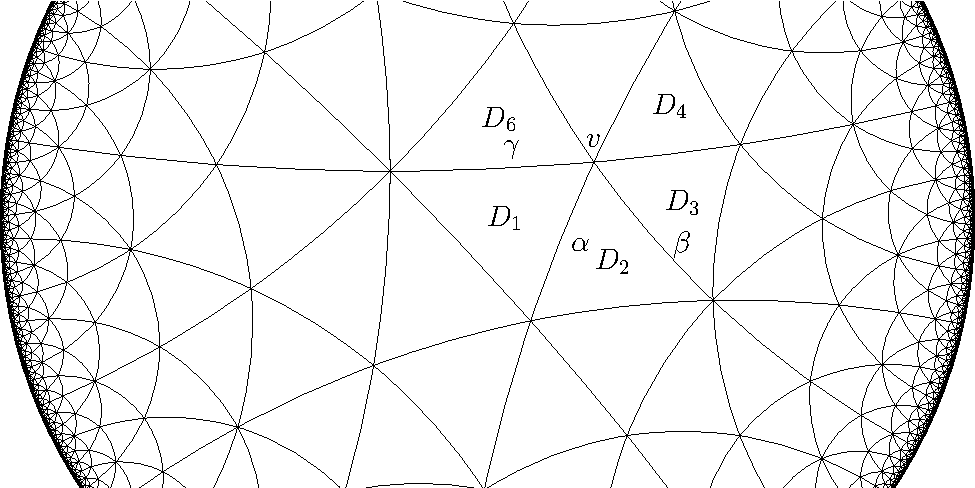
\includegraphics{diagrams/deg6433f2.pdf}
		\caption{Case: $|\st(v)|=6$}
	\end{figure}


	Now suppose $|\st(v)|=8.$ Then we will use the same labeling scheme as before except there will be $8$ chambers, and each positive root will contain exactly 4 consecutive chambers from $\st(v).$ The same logic as before will still tell us that $\gamma$ will contain exactly the chambers $D_1,D_2,D_3,D_4.$ Our first claim is that $D_2=\proj_v(C).$

	We know that $\proj_v(C)$ must lie in any positive root through $v$ and thus it can only be $D_1,D_2,D_3,D_4.$ We also know it is the chamber $A$ in $\st(v)$ which minimizes $d(A,C).$ Since $d(D_1,C)>d(D_2,C)$ we know that $D_1$ cannot be the projection. By a similar argument as before we know that $D_4$ borders $\gamma$ and thus $d(D_4,C)\ge d(D_1,C)$ by our choice of $D_1.$ Thus $D_4$ cannot be the projection. Finally, if $D_3$ were the projection then $d(D_4,C)=d(D_3,C)+1<d(D_3,C)+2=d(D_1,C)$ which is also a contradiction and thus $D_2=\proj_v(C).$

	Let $\alpha$ be the positive root separating $D_1$ and $D_2,$ $\beta$ the positive root separating $D_2$ and $D_3$ and $\delta$ the positive root separating $D_3$ and $D_4.$ Recall that $\gamma$ is the positive root separating $D_8$ and $D_1$ as well as $D_4$ and $D_5.$ We know that $D_2$ borders $\alpha$ and $\beta$ with $d(D_2,C)=d(D_1,C)-1=n-1$ and thus $\U_\alpha,\U_\beta\subset \U_{n-1}.$ 
	\begin{figure}[h]
		\label{deg8433f2}
	\begin{center}
		%\import{diagrams/}{deg8433f2}
		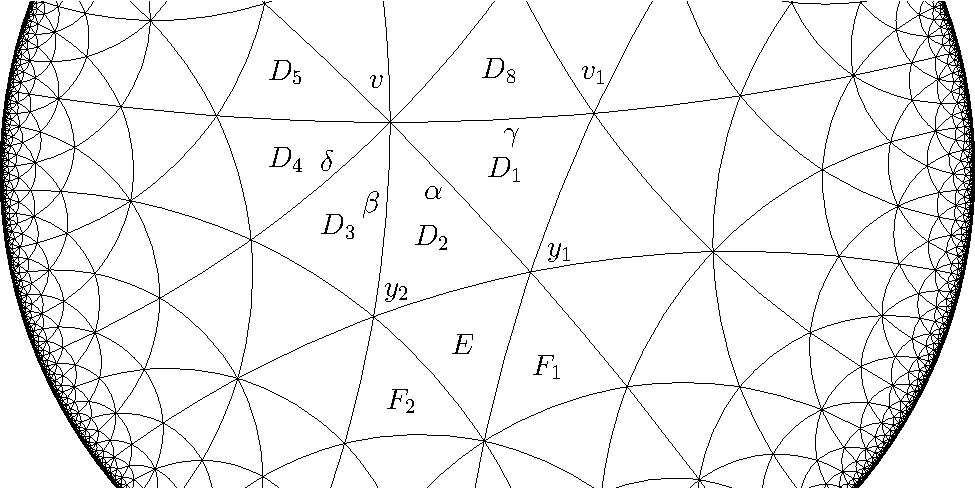
\includegraphics{diagrams/deg8433f2.pdf}
	\end{center}
	\caption{Case: $|\st(v)=8|$}
\end{figure}

Let $E$ be the third chamber adjacent to $D_2.$ Every chamber must have an adjacent chamber which is closer to $C$ and thus we have $d(E,C)<d(D_2,C).$ We can check that $d(E,C)=d(D_1,C)-2\ge 1$ by our choice of $\gamma$ and thus $E$ is not the fundamental chamber $C.$ We know that $D_1$ and $D_2$ share two vertices, and $D_2$ and $E$ share two vertices, so necessarily we have that $D_1,D_2,$ and $E$ must share at least one, and thus exactly one vertex, call it $y_1.$ By a similar argument, the chambers $D_3,D_2,$ and $E$ will also share a vertex $y_2.$ Let $F_1$ be the other chamber adjacent to $E$ that has $y_1$ as a vertex, and let $F_2$ be the other chamber adjacent to $E$ that has $y_2$ as a vertex. Note that $|\st(y_1)|=|\st(y_2)|=6$ since $v$ is the other vertex of $D_2.$ The appropriate labeling can be seen in Figure \ref{deg8433f2}, and the given diagram is unique up to a mirror image flip, which does not affect any of the following arguments. The labeling of these chambers could have simply been defined by the diagram, but the previous explanation seeks to convince the reader that no choices have been made and this diagram is unique.

Since $d(E,C)<d(D_2,C)<d(D_1,C)$ we know that there is some minimal gallery from $D_1$ to $C$ which passes through $E.$ If we fix such a minimal gallery we can see that it must pass through either $F_1$ or $F_2.$ First suppose that it passes through $F_1.$ Then $d(F_1,C)=d(D_1,C)-3$ and so $F_1$ and $D_1$ are distance 3 from one another. Since they are both in $\st(y_1),$ this means that $D_1$ and $F_1$ are opposite in $\st(y_1).$ Then there is another minimal gallery from $D_1$ to $F_1$ which does not pass through $D_2$ and can also be extended to a minimal gallery from $D_1$ to $C.$ Let $G_1$ be the chamber adjacent to $D_1$ in this new minimal gallery. Then $D_1$ and $G_1$ have exactly two vertices in common, on of which is $y_1,$ and the other cannot be $v$ as this would imply $G_1=D_2$ which contradicts our assumption. Let $v_1$ be the common vertex which is not $y_1.$ We assumed that $v$ was the unique vertex shared by $D_1$ and $D_2$ which lies on $\partial \gamma.$ Since $y_1$ is also shared by $D_1$ and $D_2$ this means that $y_1$ does not lie on $\partial \gamma.$ We assumed that $D_1$ has a panel on $\partial \gamma$ and thus it has two vertices on $\partial \gamma$ which means $v_1$ must lie on $\partial \gamma.$

Now we have the following situation. We still know that $D_1$ borders $\gamma$ with $d(\gamma,C)=d(D_1,C)$ and $G_1$ is an adjacent chamber such that $d(G_1,C)<d(D_1,C).$ We know that $v_1$ is a common vertex which lies on $\partial\gamma$ and thus it is the only common vertex which lies on $\partial\gamma.$ Finally, $v$ is the uniqe vertex of $D_1$ with 8 chambers in its star. Thus $|st(v_1)|=6.$ Now we may apply the $|\st(v)|=6$ case with $G_1$ as our new choice of $D_2$ and $v_1$ the new $v.$ This shows that $\U_\gamma\subset \U_{n-1}$ as desired.

Now suppose the fixed minimal gallery from before passes through $F_2.$ Then there is also a minimal gallery from $D_3$ to $C$ which passes through $F_2$ as well. But then $d(F_2,C)=d(D_3,C)-3$ which means $F_2$ and $D_3$ are opposite in $\st(y_2).$ Since $D_3$ borders $\delta,$ we can use similar arguments as in the previous two paragraphs to show that $\U_\delta\subset \U_{n-1}.$ However, by Lemma \ref{c2f2gen} we know that $\U_v=\langle \U_\alpha,\U_\beta,\U_\delta\rangle$ and thus $\U_\gamma\subset \U_{n-1}$ as well. Thus for any root $\gamma$ with $d(\gamma,C)=n\ge 3$ we have $\U_\gamma\subset \U_{n-1}$ and thus $\U_n\subset \U_{n-1}$ as desired.
\end{proof}

\begin{cor}
	Let $\G$ be the Kac-Moody group over $\F{2}$ with rank 3 Weyl group defined by a coxeter diagram with edge labels $3,3,4.$ Then the subgroup $\U$ is finitely generated.
\end{cor}

\subsection{Case: 336 over $\F{3}$}
I haven't typed this stuff up yet either.


\end{document}
